%; whizzy paragraph -pdf xpdf -latex ./whizzypdfptex.sh
%; whizzy-paragraph "^\\\\begin{frame}\\|\\\\emtext"
% latex beamer presentation.
% platex, latex-beamer でコンパイルすることを想定。 

%     Tokyo Debian Meeting resources
%     Copyright (C) 2012 Junichi Uekawa

%     This program is free software; you can redistribute it and/or modify
%     it under the terms of the GNU General Public License as published by
%     the Free Software Foundation; either version 2 of the License, or
%     (at your option) any later version.

%     This program is distributed in the hope that it will be useful,
%     but WITHOUT ANY WARRANTY; without even the implied warreanty of
%     MERCHANTABILITY or FITNESS FOR A PARTICULAR PURPOSE.  See the
%     GNU General Public License for more details.

%     You should have received a copy of the GNU General Public License
%     along with this program; if not, write to the Free Software
%     Foundation, Inc., 51 Franklin St, Fifth Floor, Boston, MA  02110-1301 USA

\documentclass[cjk,dvipdfmx,12pt]{beamer}
\usetheme{Tokyo}
\usepackage{monthlypresentation}

%  preview (shell-command (concat "evince " (replace-regexp-in-string "tex$" "pdf"(buffer-file-name)) "&")) 
%  presentation (shell-command (concat "xpdf -fullscreen " (replace-regexp-in-string "tex$" "pdf"(buffer-file-name)) "&"))
%  presentation (shell-command (concat "evince " (replace-regexp-in-string "tex$" "pdf"(buffer-file-name)) "&"))

%http://www.naney.org/diki/dk/hyperref.html
%日本語EUC系環境の時
\AtBeginDvi{\special{pdf:tounicode EUC-UCS2}}
%シフトJIS系環境の時
%\AtBeginDvi{\special{pdf:tounicode 90ms-RKSJ-UCS2}}

\newenvironment{commandlinesmall}%
{\VerbatimEnvironment
  \begin{Sbox}\begin{minipage}{1.0\hsize}\begin{fontsize}{8}{8} \begin{BVerbatim}}%
{\end{BVerbatim}\end{fontsize}\end{minipage}\end{Sbox}
  \setlength{\fboxsep}{8pt}
% start on a new paragraph

\vspace{6pt}% skip before
\fcolorbox{dancerdarkblue}{dancerlightblue}{\TheSbox}

\vspace{6pt}% skip after
}
%end of commandlinesmall



\title{東京エリアDebian勉強会}
\subtitle{第98回 2013年3月度}
\author{吉田俊輔\\koedoyoshida@gmail.com}
\date{2013年3月16日}
\logo{
\includegraphics[width=8cm]{image200607/openlogo-light.eps}}

\begin{document}

\frame{\titlepage{}}

\begin{frame}{設営準備にご協力ください。}
会場設営よろしくおねがいします。
\end{frame}

\begin{frame}{Agenda}
\begin{minipage}[t]{0.45\hsize}
  \begin{itemize}
  \item 注意事項
	\begin{itemize}
	 \item トイレはエレベーターホール反対側にあります。
	 \item 飲料は手動販売機があります。ゴミ箱はトイレの手前給湯室にあります。
	 \item 遅れてきた人は次に遅れてきた人を迎えに行ってください。
	\end{itemize}
 \end{itemize}
\end{minipage} 
\begin{minipage}[t]{0.45\hsize}
 \begin{itemize}
   \item 最近あったDebian関連のイベント報告
	\begin{itemize}
        \item 第96回 東京エリアDebian勉強会
        \item OSC 浜松
        \item OSC 東京
	\end{itemize}
  \item Debian Trivia Quiz
  \item 事前課題紹介
  \item ldapvi \& python-ldap で stress-free life
  \item 月刊Debhelper
  \item gdb python拡張その1
 \end{itemize}
\end{minipage}
\end{frame}


\section{イベント報告}
\emtext{イベント報告}
\begin{frame}{第96回 東京エリアDebian勉強会}
\begin{itemize}
\item 開催場所は新宿のスクエアエニックスさんでした。
\item Debian勉強会アンケート
\item 2013-2015年を妄想する
\item 月刊Debhelper
\end{itemize}
がありました。
\end{frame}
\begin{frame}{Open Source Conference 2013 Hamamatsu}
\begin{itemize}
\item 開催場所は浜松市市民協働センターさんでした。
\item 展示のみの出展で吉田、赤部さんで行いました。
\end{itemize}
\end{frame}
\begin{frame}{Open Source Conference 2013 Tokyo/Spring}
\begin{itemize}
\item 開催場所は明星大学さんでした。
\item セミナーは土曜日に「Debian Update」のタイトルで野島さんが行いました。
\item 展示は土曜のみ出展で吉田、やまねさん、杉本さんなどで行いました。
\end{itemize}
セミナー資料は下記で公開されています。
\url{http://www.ospn.jp/osc2013-spring/modules/article/article.php?articleid=5}
\url{http://tokyodebian.alioth.debian.org/2013-02.html}
やまねさんのリポートが下記にあります。
\url{http://henrich-on-debian.blogspot.jp/2013/02/open-source-conference-2013-tokyospring.html}

\end{frame}

\section{DWN quiz}
\emtext{DWN quiz}
\begin{frame}{Debian 常識クイズ}

Debian の常識、もちろん知ってますよね?
知らないなんて恥ずかしくて、知らないとは言えないあんなことやこんなこと、
みんなで確認してみましょう。

今回の出題範囲は\url{debian-devel-announce@lists.debian.org},
\url{debian-devel@lists.debian.org} に投稿された
内容とDebian Project Newsなどからです。

\end{frame}

\subsection{問題}
%; whizzy-master ../debianmeetingresume201211.tex
% $B0J>e$N@_Dj$r$7$F$$$k$?$a!"$3$N%U%!%$%k$G(B M-x whizzytex $B$9$k$H!"(Bwhizzytex$B$,MxMQ$G$-$^$9!#(B
%

\santaku
{DebConf13 $B$N3+:ECO$H3+:EF|$O!)(B}
{$BF|K\!"El5~ET(B 6$B7n(B20$BF|(B}
{$B%K%+%i%0%"(B $B%^%J%0%"(B 7$B7n(B8-14$BF|(B}
{$B%9%$%9!"%t%)!<%^%k%-%e(B 8$B7n(B11-18$BF|(B}
{3}
{$B%K%+%i%0%"$O(BDebConf12$B$N3+:ECO$G$9!#(B
DebConf13$B$O%9%$%9$N%-%c%s%WCO$G3+:E$G$9!#(B
6/20$B$O3'$5$sM=Dj$r6u$1$F$*$-$^$7$g$&!#(B}

\santaku
{$B@$3&$N(BWeb$B%5!<%P$G:G$b?M5$$N$"$k(BLinux $B%G%#%9%H%j%S%e!<%7%g%s(B(W3Techs$BD4$Y(B)$B$O!)(B}
{CentOS}
{Debian}
{Ubuntu}
{B}
{\url{http://w3techs.com/technologies/history_details/os-linux}$B$K7k2L$N%0%i%U$,$"$j$^$9!#(B
$B8=:_(B Linux $B$r;HMQ$7$F$$$k(B web $B%5!<%P$N(B 32.9\% $B$,(B Debian $B$rMxMQ$7$F$*$j!"$=$N3d9g$O8=:_$bA}2C$rB3$1$F$$$k$=$&$G$9!#(B}

\santaku
{Debian $B%+!<%M%k%A!<%`$N%a%s%P!<$G$"$j!"(Bkernel.org $B$N(B 3.2.y $B0BDjHG7ONs$N%a%s%F%J$G$b$"$k(B Ben Hutchings $B$5$s$,<!4|(B Debian $B0BDjHG$H0l=o$K=P2Y$5$l$k(B Linux $B%+!<%M%k$K(B (3.2 $B7ONs$N(B mainline $B$K$OL5$$(B) $BDI2C5!G=$,Ek:\$5$l$kM=Dj$G$"$k$H=R$Y$F$$$^$9!#(B
$BB?$/$NDI2CE@$NCf$K4^$^$l$J$$$b$N$O2?!)(B}
{PREEMPT\_RT}
{Hyper-V guest drivers$B$N6/2=(B}
{ARM64/AArch64$B%"!<%-%F%/%A%c%5%]!<%H(B}
{C}
{Hyper-V guest drivers$B$O(Bmainline kernel$B$G(B3.2$B$K$b4^$^$l$F$$$^$9$,!"$h$j2~A1$5$l$?(B3.4$B$+$i$N=$@5$,F3F~$5$l$^$9!#(B
PREEMPT\_RT$B$O%O!<%I%j%"%k%?%$%`$r<B8=$9$k$?$a$N(BPatch$B!"(B
linux-image-rt-amd64 , linux-image-rt-686-pae $B$N(Bmetapackage$B$G;HMQ$G$-$^$9!#(B
$B?7$7$$(BARM 64$B%S%C%H%"!<%-%F%/%A%c%5%]!<%H$O(Bmainline kernel 3.7$B$+$i(B}

\santaku
{Wookey$B$5$s$,%"%J%&%s%9$7$?(Balpha$BHG$N(BDebian port arm64 image$B$O!)(B}
{Debian/Ubuntu port image}
{Debian/KFreeBSD port image}
{Debian/GnuHurd port image}
{A}
{self-bootstrapp(non x86)$BBP1~$H$N$3$H$G$9!#(B\url{http://wiki.debian.org/Arm64Port}$B$G%9%F!<%?%9$,3NG'$G$-$^$9!#(B}

\santaku
{700,000$BHVL\$N%P%0$,Js9p$5$l$?F|$rEv$F$k(B700000thBugContest$B$N7k2L$,=P$^$7$?!#$=$NM=A[F|$HJs9pF|$O!)(B}
{2012/12/12$B$rM=A[$7$?(BDavidPrevot}
{$BM=A[F|(B:2013/02/04$B!"Js9pF|(B:2013/02/14}
{$BM=A[F|(B:2013/02/07$B!"Js9pF|(B:2013/02/14}
{$BM=A[F|(B:2013/02/14$B!"Js9pF|(B:2013/02/07}
{C}
{$B:G$b6a$$(B2013/02/14$B$rM=A[$7$?(BChristian Perrier$B$5$s$,Ev$F$^$7$?!#7k2L$O(B\url{http://wiki.debian.org/700000thBugContest}$B$G8x3+$5$l$F$$$^$9!#(B
$B$^$?!"(B800,000/1,000,000$BHVL\$N%P%0$,Js9p$5$l$kF|$rEv$F$k%3%s%F%9%H(B\url{http://wiki.debian.org/800000thBugContest}$B$b3+:E$5$l$F$$$^$9!#(B}

\santaku
{master.debian.org$B$,?7$7$$5!3#$K0\9T$5$l$^$7$?!#$3$l$O2?$N%5!<%P$G$7$g$&$+(B $B!)(B}
{@debian.org$B$N%a!<%k%5!<%P(B}
{$B%Q%C%1!<%8$N%^%9%?!<%5!<%P(B}
{$B%Q%C%1!<%8$N%9%]%s%5!<(B(mentor)$B$rC5$9%5!<%P(B}
{A}
{$B8E$$%5!<%P$O%G%#%9%/>c32Ey$,$"$C$?$N$G!"<wL?$HH=CG$5$l!"%G!<%?$,B;<:$9$kA0$K?7$7$$%5!<%P$K0\9T$5$l$^$7$?!#(Bftp-master.debian.org$B$O(BDebian$B$N(B official package $B%j%]%8%H%j$G$9!#%Q%C%1!<%8$N%9%]%s%5!<(B(mentor)$B$rC5$9$N$O(Bmentors.debian.net$B!#(B }

\santaku
{pbuilder$B$K(Bclang support$B$,DI2C$5$l$^$7$?!#C/$,=q$$$?%Q%C%A$G$7$g$&$+!)(B}
{Sylvestre Ledru}
{Junichi Uekawa}
{Hideki Yamane}
{C}
{Debian$B$N(BClang$B%5%]!<%H$OCe!9$H?J$s$G$$$^$9!#(B}

\santaku
{DPN - 2013$BG/(B3$B7n(B4$BF|9f$K<h$j>e$2$i$l$?F|K\$N%$%Y%s%H$O(B}
{Open Source Conference 2013 Tokyo/Spring}
{Open Source Conference 2013 Hamamatu}
{Open Source Conference 2013 Tokushima}
{A}
{\url{http://henrich-on-debian.blogspot.jp/2013/02/open-source-conference-2013-tokyospring.html} $B>\:Y$O8e$[$I!#(B}



\section{事前課題}
\emtext{事前課題}
{\footnotesize
 \begin{prework}{ dictoss(杉本 典充) }

\preworksection{Debianでここがバグってるかも?という事について列挙ください。}
squeezeのvirt-manager。KVM上で動作ている仮想マシンのコンソールを操作しているとき、キーボード操作でアンダースコアが入力できない。
\preworksection{使ったことのある/使ってみたいデバッガについて語って下さい。}
gdbとpdb(python)は使ったことがあります。コマンド単独で実行するより、EmacsのGUDモード内で動作させたほうがソースコードを見つつデバッグできるので効率がいいです。(eclipseを使ったときのような感じ)。sshしつつデバッグするときはGUIがないので必要に迫られて覚えた記憶があります。
\preworksection{LDAPのシステムを管理していますか?している場合は、slapd.confと
slapd-configどちらを使っていますか?その理由は?}
LDAPシステムの管理はしたことはありません。
\end{prework}

\begin{prework}{ キタハラ }

\preworksection{Debianでここがバグってるかも?という事について列挙ください。}
 今、ぱっと思いつかない。
\preworksection{使ったことのある/使ってみたいデバッガについて語って下さい。}
 最近、prinf とか syslog 程度で済むプログラムしか作っていないなぁ。
\preworksection{LDAPのシステムを管理していますか?している場合は、slapd.confと
slapd-configどちらを使っていますか?その理由は?}
していない。(実は大昔に、Netscape の Directory Server を・・・)
\end{prework}

\begin{prework}{ まえだこうへい }

\preworksection{Debianでここがバグってるかも?という事について列挙ください。}
Debian installer では LVMを使っているとパーティション情報を削除できず、shellモードから消してましたが、今ってどうなんでしょう。

\preworksection{使ったことのある/使ってみたいデバッガについて語って下さい。}
ちょっとgdb, pdbなど使ったことありますが、ちゃんと使ったがないのでそろそろ学習せんとあかんかなぁと思ってます。
\preworksection{LDAPのシステムを管理していますか?している場合は、slapd.confと
slapd-configどちらを使っていますか?その理由は?}
今回の発表内容なので割愛
\end{prework}

\begin{prework}{ たかはしもとのぶ }

\preworksection{Debianでここがバグってるかも?という事について列挙ください。}

 うーん、あまり思いつかないです。パッケージの設定が適切でないと思うことはありますが。

\preworksection{使ったことのある/使ってみたいデバッガについて語って下さい。}
  gdb もしくは Emacs + gdb を使ったことがあります。

\preworksection{LDAPのシステムを管理していますか?している場合は、slapd.confと
slapd-configどちらを使っていますか?その理由は?}
  管理しています。ファイルベースの方が扱いやすいので、どうしてもという場合以外は slapd.conf にしています。
\end{prework}

\begin{prework}{ yamamoto }

\preworksection{Debianでここがバグってるかも?という事について列挙ください。}

\begin{description}
\item [aptitude] (armehf と ppc64 では再現しているが、他のは大丈夫みたい?)
\#659341 なのだろうが、パッチを書けるほどは理解していない。

\item [ghc] (ppc64 だけかも知れないが、確認不可。多分 7.6.1-2 の頃からだと思う)
なんか特定のパッケージの特定位置で、ビルド中に固まる。
固まった時は buildd ユーザで、ssh と gcc のゾンビプロセスがいつも残っている。

\item [libccid] 日本では結構有名な NTTCom のカードリーダに関する typo。
1.4.6 でサポートされなくなり、1.4.8 で復活したが、その時 enbug した。
最近 wheezy に上げて気づいたが、BTS しないとと思いながらも、多忙によりまだ投げられてない。
\end{description}

\preworksection{使ったことのある/使ってみたいデバッガについて語って下さい。}
バグの状況説明で gdb で bt したことがあるぐらい。

\preworksection{LDAPのシステムを管理していますか?している場合は、slapd.confと
slapd-configどちらを使っていますか?その理由は?}
LDAP って、それおいしいの?
\end{prework}

\begin{prework}{ 野島 貴英 }

\preworksection{Debianでここがバグってるかも?という事について列挙ください。}
sid/experimental使ってるとそりゃもう遭遇します(←そのためのものですから無問題ですが)。\\
今も見る例:aptitudeがLANG=ja\_JP.utf8でこける事がある(再現条件不明)、gstreamer-pluginsで字幕が使えない(upstreamの問題?)、gnome-shellがたまにハング(upstreamの問題?)、gnome-keyringがまれにハング(upstreamの問題?)などなど。ただそれでも、結局Debianの問題じゃなくて、upstreamの問題のようなものばかり...\\
※Bug報告しろよという話もある。
\preworksection{使ったことのある/使ってみたいデバッガについて語って下さい。}
printf(笑)/gdb/perldb/pydb/adb/apd/xdebugなどなど。
\preworksection{LDAPのシステムを管理していますか?している場合は、slapd.confと
slapd-configどちらを使っていますか?その理由は?}
 秘密。slapd.conf直接編集かな。\\
理由:そんなに変更しないので、他の手段を使ってないだけだったりという消極的理由。
\end{prework}

\begin{prework}{ koedoyoshida }

\preworksection{Debianでここがバグってるかも?という事について列挙ください。}
debugイメージが標準で提供されていないこと。

\preworksection{使ったことのある/使ってみたいデバッガについて語って下さい。}
\begin{description}
\item [→使ったことがある] crash,lkst,gdb
\item [→使ってみたい] VisualStudio並みにグラフィカルなデバッグ環境
\end{description}
\preworksection{LDAPのシステムを管理していますか?している場合は、slapd.confと
slapd-configどちらを使っていますか?その理由は?}
過去の遺産のslapd.confのシステムが...
\end{prework}

\begin{prework}{ 鈴木崇文 }

\preworksection{Debianでここがバグってるかも?という事について列挙ください。}
あまりバグってると感じたことはないです。
\preworksection{使ったことのある/使ってみたいデバッガについて語って下さい。}
 gdbを使用したことがあります。emacs+gdbで使いやすい環境を作れたら使ってみたいです。統合開発環境としてのemacs+gdb連携ベストプラクティス的なものに興味があります。vim+gdbも試したことがありますが、結局gdbを直接使うようになってしまいました。
\preworksection{LDAPのシステムを管理していますか?している場合は、slapd.confと
slapd-configどちらを使っていますか?その理由は?}
LDAP使ったことないですね。
\end{prework}

}

\section{ldapvi & python-ldap で stress-free life}
\emtext{ldapvi \& python-ldap で stress-free life}


\section{月刊Debhelper}
\emtext{月刊Debhelper}

\begin{frame}{今月のコマンド}
\Large
\begin{itemize}
\item dh\_auto\_install
\item dh\_install
\end{itemize}
\end{frame}

\begin{frame}{debian パッケージ構築、全体の流れ}
\begin{enumerate}
\item パッケージビルド環境を構築する
\item 不要なファイルを削除する
\item バイナリパッケージに格納するファイルをビルドする
\item ビルドしたファイルをバイナリパッケージにまとめる
\item .changesファイルを作成する
\item パッケージに署名する
\end{enumerate}
2011年10月勉強会資料より
\end{frame}

\begin{frame}[containsverbatim]{4. ビルドしたファイルをバイナリパッケージにまとめる}
\begin{itemize}

\item 以下のdebhelper コマンドが実行されます。
\begin{commandlinesmall}
dh_testdir -> dh_auto_configure -> dh_auto_build -> dh_auto_test
-> dh_testroot -> dh_prep -> dh_installdirs -> dh_auto_install
-> dh_install -> dh_installdocs -> dh_installchangelogs
-> dh_installexamples -> dh_installman -> dh_installcatalogs
-> dh_installcron -> dh_installdebconf -> dh_installemacsen
-> dh_installifupdown -> dh_installinfo -> dh_pysupport
-> dh_installinit -> dh_installmenu -> dh_installmime
-> dh_installmodules -> dh_installlogcheck -> dh_installlogrotate
-> dh_installpam -> dh_installppp -> dh_installudev -> dh_installwm
-> dh_installxfonts -> dh_installgsettings -> dh_bugfiles -> dh_ucf
-> dh_lintian -> dh_gconf -> dh_icons -> dh_perl -> dh_usrlocal
-> dh_link -> dh_compress -> dh_fixperms -> dh_strip -> dh_makeshlibs
-> dh_shlibdeps -> dh_installdeb -> dh_gencontrol -> dh_md5sums
-> dh_builddeb
\end{commandlinesmall}
\end{itemize}
2011年10月勉強会資料より
\end{frame}

\begin{frame}{dh\_auto\_install動作解説1}

dh\_auto\_installはdebhelperのプログラムです。
自動的にファイルをパッケージ作成用のディレクトリにインストールします。
dh\_auto\_installはupstearm等のMakefileのinstallターゲット,setup.py,
Build.PLのを使用して、
インストール先はシングルバイナリ(only one binary package)であれば、
debian/package/以下です。
multiple binary packageの場合はdebian/tmp/以下になり、
その後dh\_installで適切なディレクトリに移動されます。
\includegraphics[height=3cm]{image201303/dh_auto_install1.eps}
\end{frame}

\begin{frame}{dh\_auto\_install動作解説2}
\begin{itemize}
\item 条件1:Makefile(またはsetup.pyやBuild.PL)が GNU の慣例に準拠し、\$(DESTDIR) 変数をサポートしていること。
\end{itemize}
\url{http://www.gnu.org/prep/standards/html\_node/DESTDIR.html\#DESTDIR}
\\
Makefile ファイルを変更する必要があるなら、これら \$(DESTDIR) 変数をサポートするように注意しましょう。
\begin{itemize}
\item 条件2:インストール先の指定内容が Filesystem Hierarchy Standard (FHS) に準拠していること。
\end{itemize}
\url{http://www.debian.or.jp/community/devel/debian-policy-ja/policy.ja.html/ch-opersys.html}
\end{frame}

\begin{frame}{dh\_auto\_install動作解説3}
通常プログラムのビルドに使われているmake等を使って実際のインストール先のかわりに、一時ディレクトリーの下に作成されたファイルツリーのイメージへプログラムをインストール(コピー)する。
 普通のプログラムインストールとDebian パッケージ作成というこれら二つの違いには、debhelper パッケージの dh\_auto\_configure と dh\_auto\_install のコマンドを使うことで(前述の条件を守っていれば、特に意識をせずに)対応できるはずです。
GNU autoconf を使っているプログラムは、自動的に GNU 規約に準拠するので、そのパッケージ作成は簡単にできる(はず)。
\url{http://www.debian.org/doc/manuals/maint-guide/modify.ja.html}
\end{frame}

\begin{frame}[containsverbatim]{dh\_auto\_install動作解説3}
マルチパッケージで、DESTDIRを使っていないのでoverrideで対応する例(wide-dhcpv6
\begin{commandline}
override_dh_auto_install:
        $(MAKE) prefix=$(CURDIR)/debian/tmp/usr install
\end{commandline}
この後、dh\_installで各パッケージに振り分け(後述)

\end{frame}



\begin{frame}{dh\_install動作概要}

dh\_installはパッケージ構造ディレクトリーへインストールするファイルを扱うdebhelperプログラムです。
これ以外に多くのdh\_install*コマンドが存在します。説明書(documentation),サンプル(examples),マニュアルページ(man pages)のような特定のタイプのファイルのインストールにはするにはそれら専用のプログラムの方が向いています。
\end{frame}

\begin{frame}{dh\_install*コマンド(debhelper内)}
\begin{table}[htb]
\scalebox{0.6}[0.6]{
\begin{tabular}{|l|r|} \hline
コマンド & 行数 \\ \hline
dh\_installcatalogs - install and register SGML Catalogs & 126 \\ \hline
dh\_installchangelogs - install changelogs into package build directories & 181 \\ \hline
dh\_installcron - install cron scripts into etc/cron.* & 87 \\ \hline
dh\_installdeb - install files into the DEBIAN directory & 118 \\ \hline
dh\_installdebconf - install files used by debconf in package build directories & 136 \\ \hline
dh\_installdirs - create subdirectories in package build directories & 96 \\ \hline
dh\_installdocs - install documentation into package build directories & 311 \\ \hline
dh\_installemacsen - register an Emacs add on package & 134 \\ \hline
dh\_installexamples - install example files into package build directories & 116 \\ \hline
dh\_installifupdown - install if-up and if-down hooks & 79 \\ \hline
dh\_installinfo - install info files & 87 \\ \hline
dh\_installinit - install init scripts and/or upstart jobs into package build directories & 287 \\ \hline
dh\_installlogcheck - install logcheck rulefiles into etc/logcheck/ & 76 \\ \hline
dh\_installlogrotate - install logrotate config files & 60 \\ \hline
dh\_installman - install man pages into package build directories & 268 \\ \hline
dh\_installmanpages - old-style man page installer (deprecated) & 207 \\ \hline
dh\_installmenu - install Debian menu files into package build directories & 99 \\ \hline
dh\_installmime - install mime files into package build directories & 105 \\ \hline
dh\_installmodules - register modules with modutils & 134 \\ \hline
dh\_installpam - install pam support files & 69 \\ \hline
dh\_installppp - install ppp ip-up and ip-down files & 75 \\ \hline
dh\_installtex - register Type 1 fonts, hyphenation patterns, or formats with TeX & 664 \\ \hline
dh\_installudev - install udev rules files & 125 \\ \hline
dh\_installwm - register a window manager & 118 \\ \hline
dh\_installxfonts - register X fonts & 97 \\ \hline
\end{tabular}
}
\end{table}
\end{frame}

\begin{frame}{dh\_install動作概要2}
二つの使用方法があります。
\begin{itemize}
\item upstearmのMakefileがインストールを行ってくれないとき、適所へそれらをコピーさせるために使用する。
\item 複数のバイナリパッケージを構築するラージ・パッケージを構築するとき
\end{itemize}
\end{frame}

\begin{frame}{ラージ・パッケージの構築}
(dh\_auto\_installまたはoverride\_dh\_auto\_install等を使用して)debian/tmpへすべてインストール。
そこから適切なパッケージディレクトリーを構築するためにディレクトリーやファイルをdh\_installを使用してコピーすることができます。
\\
debhelper互換性レベル7から、カレント・ディレクトリ(あるいは--sourcedirオプションで指定したディレクトリ)に対象が無ければ、dh\_installはdebian/tmpをコピー元に使用します。
\end{frame}

\begin{frame}{dh\_install動作概要3}
debian/package.installに
各パッケージへインストールするべきファイル、およびそれらがインストールされるべきディレクトリーを記載します。
フォーマットは、行単位でインストールするべきファイル(複数可)をリストし、行の末尾にそれがインストールされるべきディレクトリーを記載します。\\
要するにcpコマンドの引数です。
\\
実際にdh\_install内部ではcpコマンドが使用されています。
\end{frame}

\begin{frame}[containsverbatim]{debian/package.installの例}

\begin{commandline}
$ cat wide-dhcpv6-client.install
usr/sbin/dhcp6c
usr/sbin/dhcp6ctl
debian/dhcp6c.conf etc/wide-dhcpv6
debian/scripts/dhcp6c-script etc/wide-dhcpv6
debian/scripts/dhcp6c-ifupdown etc/wide-dhcpv6
\end{commandline}

明示的なコピー先なしで、一行に1つのファイル名あるいはワイルドカード・パターンを単独で記載すると、dh\_installが自動的に使用する目的地を推測する。
これは--autodestオプションの動作と同様。
\end{frame}

\begin{frame}[containsverbatim]{--autodest オプション}
コピー先ディレクトリを推測する。
これを指定する場合、debian/package.installファイルのコピー先ディレクトリは指定しないこと。
debian/tmpのディレクトリ配下にあるファイルをdebian/tmpを除いて
指定ディレクトリの下に対応するようにコピーする。
例 
\begin{commandline}
$ cat debian/package.install
debian/tmp/usr/bin
debian/tmp/etc/passwd
\end{commandline}
debian/tmp/usr/binをdebian/package/usr/へコピー
debian/tmp/etc/passwdをdebian/package/etc/へコピー
\end{frame}

\begin{frame}{--list-misqqsing オプション}
ファイル(およびシンボリックリンク)がどのディレクトリにもコピーされなかったときに標準エラー出力に警告を表示する。
\\
ラージ・パッケージに、新しく追加されたファイルを見逃さないためなどに使える。
\end{frame}

\begin{frame}{-Xitem, --exclude=item オプション}
指定したファイル名を含むファイルをコピー対象外とする。
\end{frame}

\begin{frame}[containsverbatim]{DEBHELPERのプログラム共通のオプション1}
アーキティクチャ独立
\begin{table}[htb]
\scalebox{0.6}[0.6]{
\begin{tabular}{|l|p{30em}|} \hline
-i, --indep & Act on all architecture independent packages. \\ \hline
\end{tabular}
}
\end{table}

例
\begin{commandline}
$ dh_make -m --rulesformat old
\end{commandline}
\begin{commandline}
install-indep:
	(中略)
        dh_prep -i 
        dh_installdirs -i
	(中略)
        dh_install -i
	(後略)
\end{commandline}
\end{frame}

\begin{frame}[containsverbatim]{DEBHELPERのプログラム共通のオプション2}
アーキティクチャ依存
\begin{table}[htb]
\scalebox{0.6}[0.6]{
\begin{tabular}{|l|p{30em}|} \hline
-s, --same-arch & This used to be a smarter version of the -a flag, but the -a flag is now equally smart. \\ \hline
-a, --arch & Act on architecture dependent packages that should be built for the build architecture. \\ \hline
\end{tabular}
}
\end{table}
例(同)
\begin{commandline}
install-arch:
	(中略)
        dh_prep -s 
        dh_installdirs -s

        # Add here commands to install the arch part 
        # of the package into debian/tmp.
        $(MAKE) DESTDIR=$(CURDIR)/debian/hello install

        dh_install -s
	(後略)
\end{commandline}
\end{frame}

\begin{frame}{DEBHELPERのプログラム共有のオプションその他1}
\begin{table}[htb]
\scalebox{0.6}[0.6]{
\begin{tabular}{|l|p{30em}|} \hline
オプション & 動作 \\ \hline
-v, --verbose & 詳しく動作を表示(Verbose mode: show all commands that modify the package build directory.) \\ \hline
--no-act & 実際の動作をしない(Do not really do anything. If used with -v, the result is that the command will output what it would have done.) \\ \hline
-ppackage, --package=package & Act on the package named package. This option may be specified multiple times to make debhelper operate on a given set of packages. \\ \hline
-Npackage, --no-package=package & Do not act on the specified package even if an -a, -i, or -p option lists the package as one that should be acted on.  \\ \hline
--remaining-packages & Do not act on the packages which have already been acted on by this debhelper command earlier (i.e. if the command is present in the package debhelper log).  For
           example, if you need to call the command with special options only for a couple of binary packages, pass this option to the last call of the command to process
           the rest of packages with default settings. \\ \hline
\end{tabular}
}
\end{table}
\end{frame}

\begin{frame}{DEBHELPERのプログラム共有のオプションその他2}
\begin{table}[htb]
\scalebox{0.6}[0.6]{
\begin{tabular}{|l|p{30em}|} \hline
オプション & 動作 \\ \hline
--ignore=file & Ignore the specified file. This can be used if debian/ contains a debhelper config file that a debhelper command should not act on. Note that debian/compat,
           debian/control, and debian/changelog can't be ignored, but then, there should never be a reason to ignore those files.
           For example, if upstream ships a debian/init that you don't want dh\_installinit to install, use --ignore=debian/init  \\ \hline
-Ptmpdir, --tmpdir=tmpdir & Use tmpdir for package build directory. The default is debian/package \\ \hline
--mainpackage=package & This little-used option changes the package which debhelper considers the "main package", that is, the first one listed in debian/control, and the one for which
           debian/foo files can be used instead of the usual debian/package.foo files. \\ \hline
-O=option|bundle & This is used by dh(1) when passing user-specified options to all the commands it runs. If the command supports the specified option or option bundle, it will
           take effect. If the command does not support the option (or any part of an option bundle), it will be ignored.\\ \hline
\end{tabular}
}
\end{table}
\end{frame}

\begin{frame}{次回発表者は?}

\Large

\center{〜さんですー}

\end{frame}

\section{gdb python拡張その1}
\emtext{gdb python拡張その1}
\begin{frame}{デバッガの使い道}
\Large
\begin{itemize}
 \item デバッグのお供に
 \item リバースエンジニアリングのお供に
\end{itemize}
\end{frame}

\begin{frame}{参考:OSSのリバースエンジニアリング}

OSSをリバースエンジニアリングしたくなる状況:

\begin{itemize}
 \item とにかく抽象化を使いこなしてるコード
 \item データドリブンなコード
 \item そもそも俺の理解を越えたコード
\end{itemize}

と戦う時。

\center{\Large ...ソースコード読んだだけでは動作がわからん... }\\

 で、デバッガで実行して動作を追いかけると、いろいろな発見があったり、動作が良くわかったり、アーキテクチャが見えたりする。
\end{frame}

\begin{frame}{gdb}

\Large
\begin{itemize}
 \item  gdbとは \\
幅広いプラットフォームで利用でき、多数のバイナリ形式に対応でき、組み込み用途にリモートデバッグまで出来る、非常に強力なデバッガ。
\end{itemize}

\end{frame}

\begin{frame}{gdb+python}
\Large
\begin{itemize}
\item gdb v7.0からgdbにpythonが合体!
\item Debian sid梱包のgdbもpythonが有効!
\end{itemize}

\center{\Large 強力なデバッガがさらに強力に!\\
gdbもこれでbattelies included!}

\end{frame}

\begin{frame}{Debian sidのgdbのpython具合}

\begin{table}[ht]
\begin{center}
\small
\begin{tabular}{|l|l|l|}
\hline
項番 & 項目 & 値 \\
\hline
1 & gdbバージョン & 7.4.1 \\
2 & pythonバージョン & 2.7.3 \\
3 & pythonサーチパス & /usr/share/gdb/python,\\
 & &/usr/lib/python2.7以下 \\
\hline
\end{tabular}
\end{center}
\end{table}

\end{frame}

\begin{frame}{ちと困る事}

\Large

 とにかく、文献が少ない!

\begin{itemize}
\item info gdb →Extending GDB→pythonの項目か、
\item \small \url{http://sourceware.org/gdb/wiki/PythonGdbTutorial}
\end{itemize}

ぐらい。
\center{他にあったら教えてーっ}

\end{frame}

\begin{frame}{補足:さらに困った事}

\Large
\center{「しまった、俺はpythonの書き方も知らなかったな。そういえば。」}\\

(即席で、文法も覚える必要がががが...)

\end{frame}

\begin{frame}[containsverbatim]{とりあえず動かしてみる}

とりあえず、動かしてみる。
(gdb)はgdbのプロンプトです。

\begin{commandline}
$gdb
(gdb) python print "hello world"
hello world
(gdb) python a=[1,2,3,4]
(gdb) python print a
[1, 2, 3, 4]
(gdb) python a.append(5)
(gdb) python print a
[1, 2, 3, 4, 5]
(gdb) python
>import sys
>print sys.path
>print sys.version_info
>ここでCtrl+d
['/usr/share/gdb/python', '/usr/lib/python2.7',
  '/usr/lib/python2.7/plat-linux2', ...中略...
\end{commandline}
% $

\end{frame}

\begin{frame}{gdb+python構造}

バックグラウンドでpython動かしてるんだろうと思ったら大間違い。
実際にはgdbにpython処理系を結合してた。

\begin{figure}[h]
\begin{center}
 \includegraphics[width=0.8\hsize]{image201301/gdb-python/gdb-python-internal-schema.eps}
\end{center}

\end{figure}

\end{frame}

\begin{frame}[containsverbatim]{module gdbの定義はどこ}

pythonでmoduleの定義を知るには、pydocがある。でも、
gdbの中に実装されたmodule gdbの定義を読むには...

\center{\Large pythonのhelp()関数を呼べばいい}

\begin{commandline}
(gdb) python help(gdb)
Help on package gdb:

NAME
    gdb

FILE
    (built-in)

PACKAGE CONTENTS
    command (package)
    printing
...中略...
\end{commandline}

\end{frame}

\begin{frame}{module gdbのclass図が見たい}
\Large

先程のmodule gdbの定義から、地道にclass図を起こしてみた。

参照:第98回東京エリアDebian勉強会資料6.6章の図参照。

\end{frame}

\begin{frame}[containsverbatim]{基本的使い方:gdbコマンドを増やす(その1)}

gdbに新規のコマンドを増やし、pythonと結合するにはgdb.Commandクラス
を継承したオブジェクトを生成して増やす。gdb側に増やすコマンド名は
gdb.Commandオブジェクトのコンストラクタ経由で登録する。

hello.pyの中身:
\begin{commandline}
import gdb                      
class HelloWorld (gdb.Command): 
  """ Greet the whole world """ 
  def __init__ (self):
     super(HelloWorld, self).__init__ ("hello-world",
                 gdb.COMMAND_OBSCURE)

  def invoke (self,arg, from_tty): 
     print "Hello, World! arg=["+str(arg)+"]"

HelloWorld() 
\end{commandline}

\end{frame}

\begin{frame}[containsverbatim]{基本的使い方:gdbコマンドを増やす(その2)}

実行してみた。

\begin{commandline}
(gdb) source hello.py
(gdb) hello-[ここでTABを押すと補完される]
(gdb) hello-world foo,bar,com
Hello, World! arg=[foo,bar,com]
(gdb) help obscure
Obscure features.

List of commands:

...中略...
hello-world --  Greet the whole world 
...中略...
\end{commandline}

\end{frame}

\begin{frame}[containsverbatim]{作ったスクリプトの自動読み込み}

いつもいつも''source スクリプト名''は面倒なので、自動で読み込ませたい時は:

\begin{itemize}
\item \verb!$(HOME)/.gdbinit!で読ませる
\item バイナリ側\verb!.gdb_gdb_scripts!セクションに埋め込む
\item ``バイナリ名''-gdb.pyという名前でスクリプトを用意する
\end{itemize}

の方法があります。

\end{frame}

\begin{frame}[containsverbatim]{.gdbinitで読ませる}

以下のファイルをHOMEディレクトリ配下に用意:
\begin{commandline}
----${HOME}/.gdbinitここから-----
source /home/foo/bar/my-gdb-func.py
----${HOME}/.gdbinitここまで-----
\end{commandline}
\end{frame}

\begin{frame}[containsverbatim]{.gdb\_gdb\_scriptsで読ませる}

以下のasm命令を打ち込んでおく。
\begin{commandline}
asm(
".pushsection \".debug_gdb_scripts\",\"MS\",@progbits,1\n"
".byte 1\n"
".asciz \"hello.py\"\n"
".popsection \n"
);
\end{commandline}

\center{\Large ちと脆弱性の香りが...}

\end{frame}

\begin{frame}[containsverbatim]{``バイナリ名''-gdb.pyで読ませる}

\begin{commandline}
$ ls 
hello hello-gdb.py hello.c
\end{commandline}
%$

gdb helloとすると、hello-gdb.pyが自動で読み込まれる。

\end{frame}

\begin{frame}[containsverbatim]{基本的使い方:breakpointを操る}

gdb.Breakpoint クラスを継承したオブジェトを用意すると、
指定したbreakpointで特定の処理をさせる事が可能。

mainでbreakしてhi!と表示する例:
\begin{commandline}
class _ExampleBreakpoint(gdb.Breakpoint):
   def __init__(self, spec):
       super(_ExampleBreakpoint, 
            self).__init__(spec,gdb.BP_BREAKPOINT,
                          internal = False)
   def stop(self):
        print "hi!"

_ExampleBreakpoint("main")
\end{commandline}

gdb.BP\_BREAKPOINTを指定すると、breakpointになり、
gdb.BP\_WATCHPOINTを指定すると、watchpointとなる。
\end{frame}

\begin{frame}[containsverbatim]{基本的使い方:finishを操る}

gdb.FinishBreakpoint クラスを継承したオブジェトを用意すると、
現在のスタックフレームから飛び出ようとするとbreakする。

スタックフレームから出るとhi!と表示する例:
\begin{commandline}
class _ExFinishBreakpoint(gdb.FinishBreakpoint):
   def __init__(self):
        super(_ ExFinishBreakpoint, 
              self).__init__(internal=False)
   def stop(self):
        print "hi!"

   def out_of_scope(self):
        print "hi!"
\end{commandline}

stop()は、returnによりスタックフレームから出る場合、out\_of\_scope()はlongjumpとか
で一機に飛び出す場合にbreakする。

\end{frame}

\begin{frame}[containsverbatim]{基本的使い方:コマンドの結果を得る}

gdbのコマンドの実行結果を得る事ができると便利な場合があります。

\begin{commandline}
result=gdb.execute('info break',False,True)
\end{commandline}

resultにgdbのコマンド''info break''の結果が文字列クラスで格納されます。

\end{frame}

\begin{frame}{以上を活用してみた例}

 解析用途で、プログラムのコールツリーを取ってみたかった。

 具体的なスクリプトのソースと使い方は、\\
第98回東京エリアDebian勉強会資料6.9章参照。

\end{frame}

\begin{frame}{calltracer.py動作説明}

\begin{description}
\item [Step 1.] rbreakを実行して、デバッグ情報にある全関数に一旦breakpointを仕掛ける
\item [Step 2.] info breakの結果をパースして、関数のアドレスと、名前の両方を得る。
\item [Step 3.] カスタマイズしたbreakpointと入れ替える。
\item [Step 4.] breakしたら、スタック追跡変数(self.stack)を+1して関数名を表示。同時にカスタマイズしたfinishを仕掛ける。
\item [Step 5.] finishでbreakしたら、関数名を表示してスタック追跡変数を-1する。
\item [Step 6.] Step 4.〜Step 5.を繰り返す。
\end{description}

\end{frame}

\begin{frame}{終わりに}

\center{\Large pythonのおかげで、\\なんかもう夢ひろがりんぐ\\
まだまだ機能満載なので、\\次回も発表続けるよどこまでも!}

\end{frame}

\section{今後のイベント}
\emtext{今後のイベント}
\begin{frame}{今後のイベント}
\begin{itemize}
 \item 2013年4月 Debian勉強会
\end{itemize}
\end{frame}

\section{今日の宴会場所}
\emtext{今日の宴会場所}
\begin{frame}{今日の宴会場所}
未定
\end{frame}

\end{document}

;;; Local Variables: ***
;;; outline-regexp: "\\([ 	]*\\\\\\(documentstyle\\|documentclass\\|emtext\\|section\\|begin{frame}\\)\\*?[ 	]*[[{]\\|[]+\\)" ***
;;; End: ***
